\documentclass[12pt]{article}
\usepackage{graphicx}
\usepackage{caption}
\usepackage[margin=.75in]{geometry}
\usepackage{float}
\usepackage[export]{adjustbox}
\usepackage{amsmath}
\usepackage{epstopdf}
\usepackage{subcaption}
\usepackage{amssymb}

\begin{document}

\title{Automatic Verification of Nonlinear Systems without Abstractions Using Continuation Methods}
\date{}
\author{}
\maketitle

\begin{figure}[h]
\begin{center}

\includegraphics[width=3.5in]{uw_logo.png}
\end{center}
\vspace{-0.25in}
\end{figure}

\begin{center}
\textbf{Peter Uth}\\Research Assistant\\William E. Boeing Department of Aeronautics \& Astronautics\\University of Washington\\Phone: (774) 254-2508, Email: puth@uw.edu
\end{center}

\begin{center}
\textbf{Anshu Narang-Siddarth}\\Assistant Professor\\William E. Boeing Department of Aeronautics \& Astronautics\\University of Washington\\Phone: (206) 543-6679, Email: anshu@aa.washington.edu
\end{center}

\vspace{0.5in}

\begin{figure}[h]
\begin{center}

\includegraphics[width=1.5in]{afrl_logo.png}
\end{center}
\vspace{-0.25in}
\end{figure}

\begin{center}
\textbf{Matthew Clark}\\Chief, Autonomous Control Branch\\Air Force Research Laboratory AFRL/RQQA\\Phone: 937-713-7004, Email:  matthew.clark.20@us.af.mil
\end{center}

\newpage

\section{Introduction}

Assuring safe performance of a system is a critical component of the design process. An analysis of a system's underlying dynamics can result in the detection of unsafe properties early in the process, thus avoiding more expensive design changes in later stages of development. However, a complete understanding of nonlinear system dynamics is typically difficult to obtain due to the wide range of possible behavior. This presents a fundamental challenge to ensuring safe operation, particularly for highly autonomous systems with large sets of possible operating conditions. As advances in autonomy yield more intelligent and complex systems, the common practice of verifying safety properties by performing a time simulation for every possible set of operating conditions becomes inadequate. Verification and validation (V\&V) architectures that employ model checking or theorem proving techniques can provide an exhaustive means of verifying safety properties. However while these techniques are useful, they are restrictive in the class of systems they can handle and are often computationally intensive. Therefore, new V\&V techniques are required to keep pace with the development of increasingly intelligent and diverse systems. 

Numerical continuation methods can be used to characterize how the behavior of a system changes as parameters are varied via a bifurcation analysis \cite{allgower}. The term bifurcation defines a point in state-parameter space for a dynamical system where changes occur in the number and/or stability of equilibrium solutions \cite{Strogatz}. The results of a numerical continuation analysis, typically a bifurcation diagram depicting the equilibrium solution branches and their stability, provide insight on safe and unsafe operating conditions for the system being analyzed.

While bifurcation diagrams are useful representations of system behavior, they do not lend themselves to an automatic verification scheme and they do not explicitly define stable/unstable (i.e. safe/unsafe) regions of the operational envelope. Capturing the basins of attraction (i.e. the domain of initial conditions for which trajectories will reach a stable equilibrium as $t \to \infty$) of the continuation data would enable the direct determination of safe/unsafe domains of the system state-space. Using this information, a system representation based on safe/unsafe operating conditions with identified domains would be well-suited for automatic safety verification and would provide a useful visualization of system behavior. Additionally, this type of representation could interface with verification schemes such as model checking and theorem proving to enhance their capabilities. 

A continuation-based approach to safety verification can provide advantages in flexibility and computational efficiency over existing methods. The overall goal of this work is to leverage these advantages to create a safety analysis framework and integrate with existing methods to support a more comprehensive V\&V architecture. This is itemized into the following subgoals:

\begin{itemize}
\item Use numerical continuation to obtain information on system equilibria, including the stability and basin of attraction for each equilibrium. This information translates into safe and unsafe domains of the operational envelope.
\item Create a graphical representation framework that separates system behavior into subsystem nodes based on stability information gathered from the continuation analysis. Define transition conditions between nodes to capture when major changes in system behavior occur.
\item Incorporate this representation into existing V\&V schemes, such as model checkers and/or theorem provers. 
\end{itemize}

This paper documents the continuing progress made towards these goals. It begins with background information on important concepts. Then, a section is added to the end of this document for each status update.


\section{Background}

\subsection{Numerical continuation}
\label{continuation}
Numerical continuation methods seek to find solution sets of vector $z$ to underdetermined nonlinear equations in the form of 
\begin{equation}
\label{eq1}
F(z)=0, \qquad F:\mathbb{R}^{n+1} \to \mathbb{R}^n.
\end{equation}
Sets of solutions $z$ form solution branches. Continuation numerically approximates these solution branches through predictor and corrector iterations. The process is as follows. First, an initial point on the solution curve is identified. Then, a prediction is made from the initial point by moving a step size $h$ in the direction tangent to the solution at the initial point. This direction is determined by calculating the Jacobian matrix $F_z=\frac{\partial F}{\partial z}$. Next, a corrector is applied to increase the accuracy of the predicted point until a defined tolerance is reached. A Newton-type corrector method is commonly used. The newly obtained corrected point is then used as the next initial point and the process is repeated. These predictor-corrector steps are iterated to create a solution branch. This process is illustrated in Figure \ref{continuation_allgower}, where $u_i$ is the initial point, $v_{i+1}$ is the predicted point, $u_{i+1}$ is the corrected point, and $w_{i+1}$ is the target point on the original nonlinear solution branch \cite{allgower}.

\begin{figure}[h]
\begin{center}
 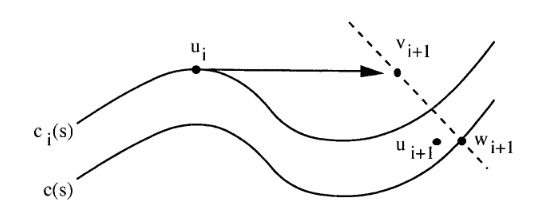
\includegraphics[width=3.75in]{continuation_allgower.png}
 \caption{Continuation process illustrated.}
 \label{continuation_allgower}
 \end{center}
\end{figure}

COSY \cite{spetzler} is a numerical continuation tool for MATLAB that allows for the inclusion of equality constraints and is used for the work described in this paper. 


\subsection{Bifurcation analysis}
Bifurcation analyses typically investigate dynamical systems of the form 

\begin{equation}
\label{bf1}
\dot{x}=f(x,p),
\end{equation}
where $x$ is the vector of system states and $p$ is a parameter. Equilibrium points occur at sets of $x$ and $p$ that solve $\dot{x}=f(x,p)=0$. Therefore, equilibrium properties are dependent on system behavior at values of $p$. Numerical continuation determines these properties by finding solution sets as parameter $p$ is varied using the process outlined in Section \ref{continuation} and equation (\ref{eq1}) with 

\begin{equation}
\label{bf2}
F(z)=f(x,p).
\end{equation}
The result is information on the number and location of equilibria for different values of parameter $p$. Additionally, the stability of each equilibrium is determined by observing the Jacobian matrix for each step of the continuation process (i.e. negative values indicate stable while positive values indicate unstable). Typical bifurcation types include, but are not limited to, the following:

\begin{itemize}
\item \textbf{Saddle node bifurcations} occur when two equilibrium points annihilate each other for some value of parameter $p$. For example, the dynamical system 
\begin{equation}
\label{bf3}
\dot{x}=p+x^2
\end{equation}
experiences a saddle node bifurcation at $p=0$. When $p<0$ there are two solutions to $\dot{x}=0$, but when $p>0$ these solutions disappear. 
\item \textbf{Pitchfork bifurcations} occur when a transition is made from a single equilibrium point to three equilibrium points for some value of parameter $p$. For example, the dynamical system 
\begin{equation}
\label{bf4}
\dot{x}=px-x^3
\end{equation}
experiences a pitchfork bifurcation at $p=0$. When $p<0$, only one equilibrium exists at $x=0$. When $p>0$, $x=0$ remains and two additional equilibria appear.
\item \textbf{Transcritical bifurcations} occur when two equilibrium points switch their stability. For example, the dynamical system 
\begin{equation}
\label{bf5}
\dot{x}=px-x^2
\end{equation}
experiences a transcritical bifurcation at $p=0$. The two equilibrium points are always at $x=0$ and $x=p$. When $p<0$, $x=0$ is stable and $x=p$ is unstable. When $p>0$, $x=0$ is unstable and $x=p$ is stable.
\end{itemize}


\subsection{V\&V tools}
\subsubsection{Model checking}
The term model checking describes techniques to automatically verify the correctness of finite-state systems \cite{Clarke1,Clarke2}. The inputs to a model checker are mathematical representations of the system to be verified and the property specifications, typically expressed as logic formulas, that are used to determine correctness. Model checkers then apply exhaustive search algorithms to the entire state-space to determine if the property specifications hold true or are violated. For increasingly complex systems, an exponential growth of this exhaustive search process leads to a state-space explosion problem. Therefore, model checkers require abstraction of the target system to ease the computational process \cite{Clarke3,Merz}. This sacrifices fidelity to the original system and often necessitates a separate review process to ensure that the abstracted model adequately reflects the original system. 


\subsubsection{Theorem proving}
Theorem proving, or automated reasoning, is a commonly used verification method \cite{Hasan,Harrison}. Mathematical models of the system and the property specification must be formalized into a logic-based architecture. Typical theorem provers work by expanding on well-known axioms to deduce the validity of the specification for the system being verified. The logic formalization restricts the capabilities of theorem proving, with trade-offs between system complexity and automation potential dependent on the level of logic expression. Propositional logic expression is very limited in the types of systems that can be expressed, but is easily incorporated into automated verification schemes. First-order logic has fewer limitations on system expressions, but may require some user interaction. Higher-order logic can be used to express complex systems, but is highly user-interactive and therefore not suitable for automatic verification.


\section{Status updates}
This section details progress made and concerns raised for this project. Note that the January 13, 2017 section summarizes the work that was completed prior to the creation of this document.

\subsection{January 13, 2017}
\label{jan13}
A graph representation is proposed where each equilibrium is depicted by a node. Each node is identified as stable or unstable with an identified domain. The domain of a stable node is defined as its basin of attraction, while the domain of an unstable node is defined as a region where unstable behavior is observed. Transitions from one node to another is depicted by arrows labeled with the transition conditions. The proposed process to generate a graph representation of a system is as follows:
	
\begin{enumerate}
  \item Numerical continuation is used on the input system dynamics to generate data on the equilibrium solution branches, including their stability and domains.
  \item The continuation output information, typically presented as a bifurcation diagram, is converted to a graph description language (e.g. DOT \cite{Koutsofios}). If the user specifies a value of interest for parameter $p$, only data for that particular $p$ will be converted.
  \item A graph visualization tool (e.g. GraphViz \cite{Ellson}) reads the DOT file and generates a graph representation.
\end{enumerate}

A graph representation concept of data from a bifurcation diagram is shown in Figure \ref{jan13_graph_concept}. The stable and unstable equilibrium branches shown in the bifurcation diagram are represented as nodes. An additional node represents the region of $p>0$ where no equilibrium branches exist. Transitions between nodes are labeled with the appropriate $x$ and $p$ domains. In Figure \ref{jan13_graph_concept}, $D_s(p)$ and $D_u(p)$ are stable and unstable $x$ domains, respectively, which are dependent on the value of $p$. Cases where $p$ is an unspecified value, such as in Figure \ref{jan13_graph_concept}, are referred to as ``general'' while cases with a user-specified value for $p$ are referred to as ``fixed-$p$.'' An automated process for fixed-$p$, 1-variable systems along with concept examples of the graph representation for typical saddle node and pitchfork bifurcation cases are shown in the following sections. 

\begin{figure}[H]
\begin{center}
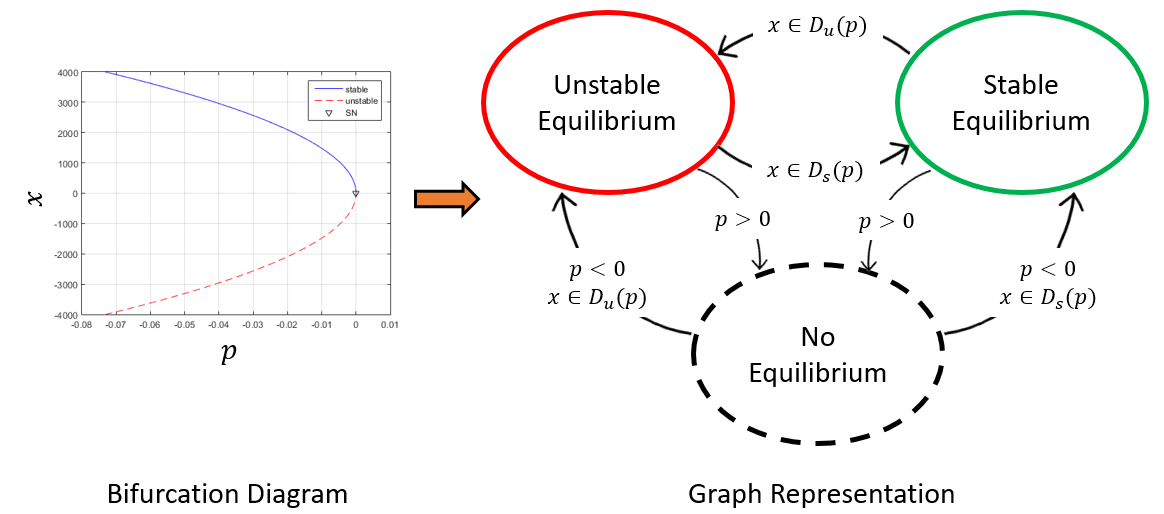
\includegraphics[width=6in]{jan13_graph_concept.png}
\caption{A bifurcation diagram (left) and corresponding graph representation concept (right).}
\label{jan13_graph_concept}
\end{center}
\end{figure}


\subsubsection{1-variable, fixed-$p$ automated process}
\label{process_1var}
An automated process was created in MATLAB that follows the generalized steps from section \ref{jan13} for 1-variable, fixed-$p$ cases:

\begin{enumerate}
\item Identify system equation, variable $x$, parameter $p$, limits, and any other options for the COSY continuation tool.
\item Run COSY. This will produce equilibrium solution branches for the system with stability information.
\item Identify the domain for each equilibrium branch. This is not an output of COSY and thus requires a post-processing step. For fixed-$p$ cases, these equilibrium branches are reduced to the equilibrium points along the branches at the specified value of $p$. The process for identifying the equilibrium domains for 1-variable, fixed-$p$ cases is as follows:
	\begin{enumerate}
	\item If no equilibrium exists, no domains are identified.
	\item If only one equilibrium exists, its domain is all values of $x$, or $x\in [-\infty \quad +\infty]$.
	\item For multiple equilibria, the first equilibrium (E1) has the lowest $x$-value. Since no equilibrium exists below this, the lower limit of the domain for E1 is $-\infty$. 
	\item If E1 is unstable then the upper limit of its domain is its $x$-value since any trajectories starting above this value will trend towards the second equilibrium (E2), which is stable. If E1 is stable then the upper limit of its domain is the $x$-value for E2, which is unstable. This method takes advantage of the fact that in 1-variable systems, the stability of an equilibrium point is opposite the stability of the adjacent equilibrium points \cite{Strogatz}. For example, the stability ordering for a system with three equilibrium points is either stable-unstable-stable or unstable-stable-unstable.
	\item This process is repeated for E2 and beyond, with the domain determined by using the stability of the equilibria above and below. 
	\item The upper domain for the highest $x$-value equilibrium is +$\infty$.
	\end{enumerate}
\item Each equilibrium, along with stability and domain, is constructed into a node definition written in DOT syntax. 
\item A DOT file is created with all node information. Labels for the transitions between nodes are added to this file.
\item GraphViz is executed on the DOT file and a PNG image file is displayed containing the graph representation.
\end{enumerate}


\subsubsection{Saddle node bifurcation}
A typical saddle node bifurcation can be observed with the equation

\begin{equation}
\dot{x}=p+x^2.
\end{equation}
Using the COSY continuation tool, the solution branches to $\dot{x}=0$ while varying $x$ and parameter $p$ as active continuation parameters is shown in Figure \ref{jan13_bfd_sn1}. An unstable equilibrium branch can be seen in the domain of positive $x$ and a stable equilibrium branch in the domain of negative $x$. A saddle node bifurcation occurs at $p=x=0$, since the two equilibrium branches appear when $p$ crosses into the negative domain and disappear when $p$ crosses into the positive domain.

\begin{figure}[H]
\begin{center}
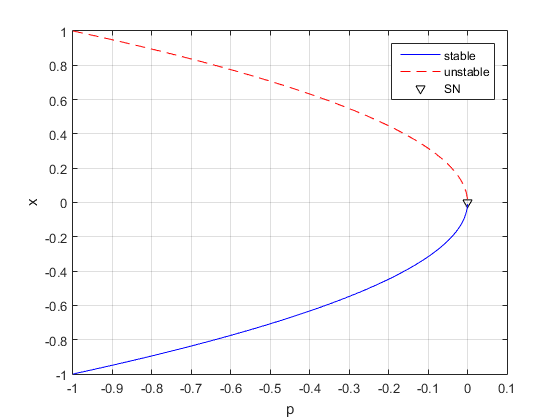
\includegraphics[width=3.5in]{jan13_bfd_sn1.png}
\caption{Continuation output a showing saddle node bifurcation at (0,0).}
\label{jan13_bfd_sn1}
\end{center}
\end{figure}

A graph representation concept of the data shown in Figure \ref{jan13_bfd_sn1} for the general case is shown in Figure \ref{jan13_graph_sn1}. The three nodes represent the stable equilibrium branch, the unstable equilibrium branch, and the region of positive $p$ where no equilibria exist. Note that Figure \ref{jan13_graph_sn1} was generated by manually writing a GraphViz-compatible DOT file for concept purposes. For a fixed-$p$ case, the graph simplifies to describe only equilibrium data that can exist for the specified $p$. Figure \ref{jan13_graph_sn2} shows the graph representation for fixed-$p$ cases of -0.5 and +0.5. Note that Figure \ref{jan13_graph_sn2} was generated using the automated process previously described in Section \ref{process_1var}.

\begin{figure}[H]
\begin{center}
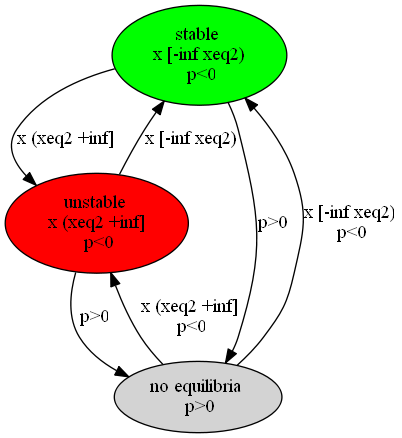
\includegraphics[width=2.75in]{jan13_graph_sn1.png}
\caption{Graph representation of a typical saddle node bifurcation for the general case. ``xeq2'' is the $x$ value of the unstable equilibrium and is undefined since $p$ is not specified.}
\label{jan13_graph_sn1}
\end{center}
\end{figure}

\begin{figure}[H]
\begin{center}
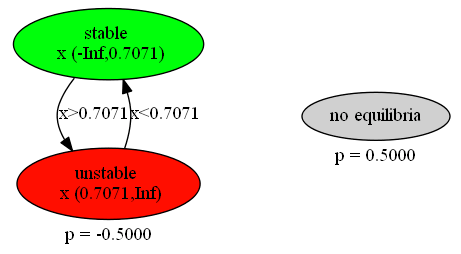
\includegraphics[width=3.5in]{jan13_graph_sn2.png}
\caption{Graph representation of a typical saddle node bifurcation for fixed-$p$ cases of -0.5 (left) and +0.5 (right).}
\label{jan13_graph_sn2}
\end{center}
\end{figure}

\subsubsection{Pitchfork bifurcation}
A typical pitchfork bifurcation can be observed with the equation

\begin{equation}
\dot{x}=px-x^3.
\end{equation}
Using the COSY continuation tool, the solution branches to $\dot{x}=0$ while varying $x$ and parameter $p$ as active continuation parameters is shown in Figure \ref{jan13_bfd_pf1}. One stable equilibrium exists for negative $p$, while two stable and one unstable equilibria exist for positive $p$. Therefore it can be seen that a pitchfork bifurcation occurs at $p=x=0$.

\begin{figure}[H]
\begin{center}
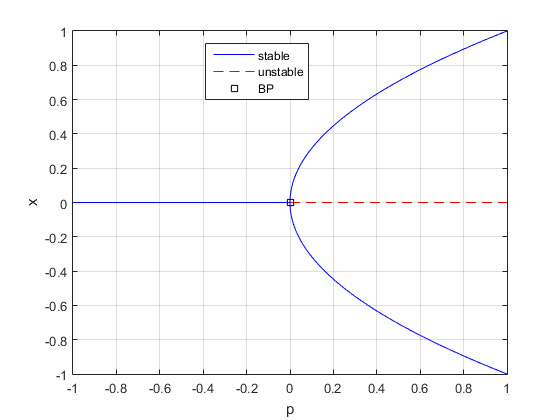
\includegraphics[width=3.5in]{jan13_bfd_pf1.png}
\caption{Continuation output showing a pitchfork bifurcation at (0,0).}
\label{jan13_bfd_pf1}
\end{center}
\end{figure}

A graph representation of the data shown in Figure \ref{jan13_bfd_pf1} for fixed-$p$ cases of -0.5 and +0.5 is shown in Figure \ref{jan13_graph_pf2}. When $p$ is positive, the equilibria are depicted as two stable nodes and one unstable node. The domain for the unstable node is only $x=0$ since moving away from this value will result in attraction to one of the stable nodes. When $p$ is negative, there is a single stable node with the domain of all $x$ values. Note that Figure \ref{jan13_graph_pf2} was generated using the automated process previously described in Section \ref{process_1var}.

\begin{figure}[H]
\begin{center}
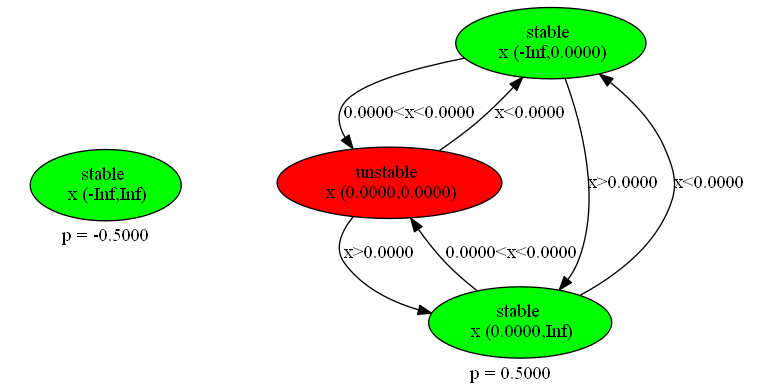
\includegraphics[width=5in]{jan13_graph_pf2.png}
\caption{Graph representation of a typical pitchfork bifurcation for fixed-$p$ cases of -0.5 (left) and +0.5 (right).}
\label{jan13_graph_pf2}
\end{center}
\end{figure}


\subsubsection{Questions/concerns}
\begin{itemize}
	\item The automated process discussed in Section \ref{process_1var} currently works for fixed-$p$ cases but not general cases. Since the general case is important for representing the behavior of the entire system, this process will be extended to work for general cases with outputs similar to Figure \ref{jan13_graph_sn1}.
	\item This method of analysis and graph generation is currently set up to handle systems with one variable $x$ and one parameter $p$. It is planned to extend these capabilities to handle multivariate systems. This will require a much more complex analysis, particularly for determining equilibrium domains when the 1-variable stability behavior as discussed in Section \ref{process_1var} cannot be used.
\end{itemize}


\subsection{January 20, 2017}
\label{jan20}
The graph representation style previously discussed was restructured into top level $p$-nodes that contain sub level $x$-nodes. The $p$-nodes are defined by domains of $p$ that represent different behaviors. For example, if a bifurcation (i.e. a change in equilibrium nodes) occurs at $p=0$, two $p$-nodes are generated: one for $p<0$ and one for $p>0$ (i.e. on either side of the bifurcation point). Within these two $p$-nodes are the stability nodes defined by domains of $x$, similar to the original graphs shown in Section \ref{jan13}. Examples of this graph representation for the typical saddle node and pitchfork bifurcation cases are shown in Figures \ref{jan20_graph_sn} and \ref{jan20_graph_pf}. General and fixed-$p$ cases are displayed. The $p$-nodes are depicted by the black rectangular outlines and the $x$-nodes by the colored ovals. The domain of $p$ and the relevant equilibrium equation are shown at the top of each $p$-node. Note that for the general cases the equations are simply the original equation with $\dot{x}=0$, which defines the equilibria, since $p$ is not defined. The original equations are displayed at the bottom of the graphs. For the fixed-$p$ cases, the specified value for $p$ is also at the bottom. Also for the fixed-$p$ cases, the $p$ domain is still shown (e.g. $p<0$) to provide information on when the graph is no longer valid (i.e. when the node configuration will change from what is shown). Note that Figures \ref{jan20_graph_sn} and \ref{jan20_graph_pf} were manually generated in the DOT language for conceptual purposes. 

\begin{figure}[H]
\centering
\begin{subfigure}[b]{0.35\textwidth}
	\centering
	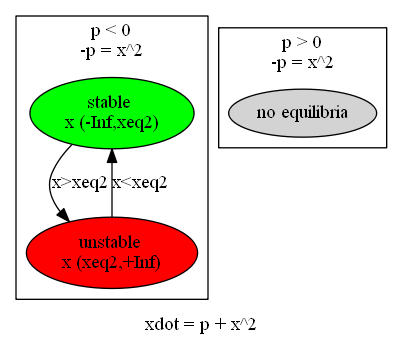
\includegraphics[width=3in]{jan20_graph_sn1.png}
	\caption{General $p$}
	\label{jan20_graph_sn1}
\end{subfigure}
\qquad \qquad
\begin{subfigure}[b]{0.4\textwidth}
	\centering
	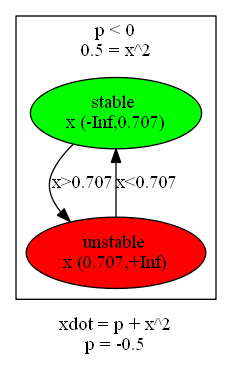
\includegraphics[width=1.75in]{jan20_graph_sn2.png}
	\caption{Fixed $p$}
	\label{jan20_graph_sn2}
\end{subfigure}
\caption{Graph representation of a typical saddle node bifurcation for general and fixed-$p$ cases.}
\label{jan20_graph_sn}
\end{figure}

\begin{figure}[H]
\centering
\begin{subfigure}[b]{0.4\textwidth}
	\centering
	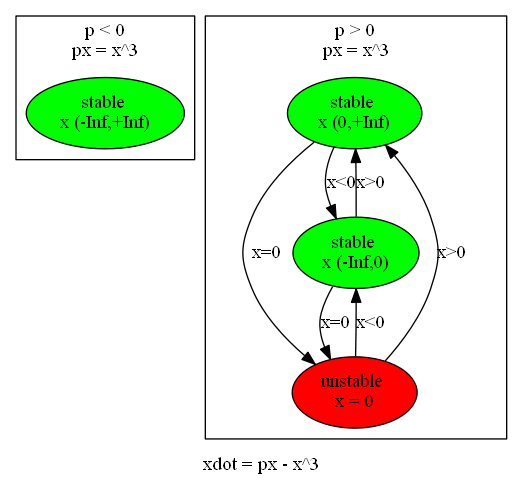
\includegraphics[width=3.75in]{jan20_graph_pf1.png}
	\caption{General $p$}
	\label{jan20_graph_pf1}
\end{subfigure}
\qquad \qquad
\begin{subfigure}[b]{0.4\textwidth}
	\centering
	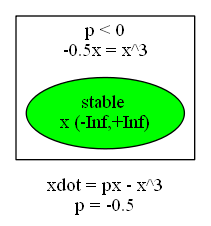
\includegraphics[width=1.5in]{jan20_graph_pf2.png}
	\caption{Fixed $p$}
	\label{jan20_graph_pf2}
\end{subfigure}
\caption{Graph representation of a typical pitchfork bifurcation for general and fixed-$p$ cases.}
\label{jan20_graph_pf}
\end{figure}

\subsubsection{Questions/concerns}
\begin{itemize}
\item Figures \ref{jan20_graph_sn} and \ref{jan20_graph_pf} were manually generated in the DOT language. It is desired to automate this process similar to what was presented in Section \ref{process_1var} for both the general and fixed-$p$ cases (previous automated process did not work for the general cases).
\end{itemize}


\subsection{February 3, 2017}
An automated process for generating the graph representation discussed in Section \ref{jan20} for fixed-$p$ cases was created. This process is similar to the process described in Section \ref{process_1var} but now includes the top level $p$-nodes with sub level $x$-nodes structure. Additionally, the code for this process, which was previously a preliminary test script, was constructed into a MATLAB function file. The inputs to this function are the dynamic equation, the solution branch data from the continuation analysis, the specified $p$ value, and the desired label for the graph output. Therefore the use of this function requires the COSY continuation process to be completed first. The continuation and graph generation processes may be combined later so that the user only has to call one function. 

\subsubsection{Questions/concerns}
\begin{itemize}
\item The automated graph generation process only works for fixed-$p$ cases. The next step is to extend these capabilities to general cases. 
\item The short term goal is to have a complete function that can handle 1-variable cases (both fixed-$p$ and general) before moving on to the more challenging multivariate cases.
\end{itemize}


\subsection{February 10, 2017}
Progress was made on the automated process for general cases. The algorithm begins by separating the continuation output data into different domains of parameter $p$. These domains are identified using ``events'' in the data, such as bifurcation points, and are used to define the top level $p$-nodes of the graph representation. The number and stability of solution branches within each $p$-domain is then used to create the stable and unstable $x$-nodes. The current graph representation output is shown in Figure \ref{feb10_graph_pf1}. Note that the general case process is only partially complete and therefore the representation shown is lacking certain details that will be added later (e.g. transition conditions).

\begin{figure}[H]
\begin{center}
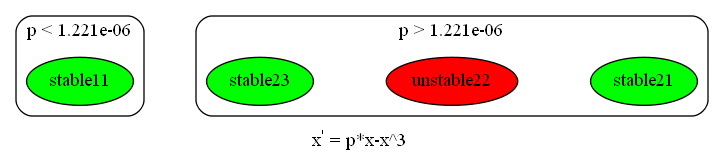
\includegraphics[width=5in]{feb10_graph_pf1.png}
\caption{Work-in-progress graph representation of a typical pitchfork bifurcation for the general case.}
\label{feb10_graph_pf1}
\end{center}
\end{figure}

\subsubsection{Questions/concerns}
\begin{itemize}
\item The automated process for the general case requires completion and refinement. The pitchfork bifurcation case has been used to test the algorithm, but other cases must also be tested after a baseline process is complete. For example the ``no equilibria'' node, which does not exist in the pitchfork case, will have to be incorporated for saddle node and other cases.
\end{itemize}


\subsection{February 17, 2017}
Further progress was made on the automated process for general cases. The current graph representation output for the pitchfork bifurcation case is shown in Figure \ref{feb17_graph_pf1}. Since the last update, domain identification and $x$-node transition arrows have been added to the algorithm. However additional detail still needs to be added (e.g. transition conditions). 

\begin{figure}[H]
\begin{center}
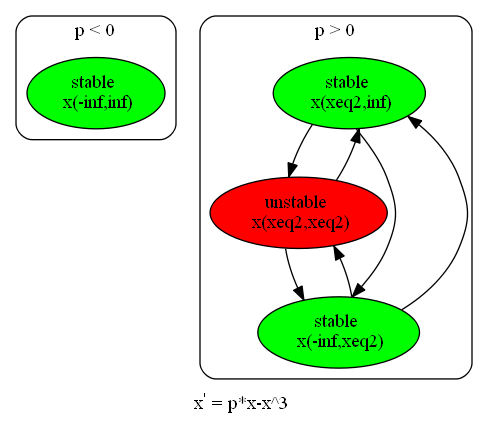
\includegraphics[width=3in]{feb17_graph_pf1.png}
\caption{Work-in-progress graph representation of a typical pitchfork bifurcation for the general case.}
\label{feb17_graph_pf1}
\end{center}
\end{figure}

In addition to the development of a verification-friendly graph representation as presented so far, the capability of using continuation methods to break down a complex system into simpler dynamic nodes was discussed. Section \ref{VOO_01} documents this discussion. To summarize, it is desired to take the equation(s) for a complex system and separate into simpler nodes by adjusting certain parameters and applying the continuation methods previously discussed. The output would be a hybrid graph representation that captures an original complex system's dynamics within a series of nodes containing more manageable dynamics. Proposed next steps towards this goal were identified as follows:

\begin{enumerate}
\item Automatically create the ``irreducible'' hybrid model using continuation methods. The automated graph representation process under development is targeting this goal. The 1-parameter, simple bifurcation cases investigated so far are considered ``irreducible,'' where as a ``reducible,'' more complex system would break down into nodes similar to the simple cases.
\item Add representative variables to the simple cases to explore how more complex systems can be broken down. For example, change $\dot{x}=p_1+x^2$ to $\dot{x}=p_1+p_2x^2$ to see how the addition of $p_2$ changes the hybrid system.
\item Add more dimensions (i.e. systems of equations with multiple variables $x$). 
\item Add more nonlinearities (e.g. sin, cos, etc.).
\end{enumerate}

The concept of this process would iteratively alter parameters and apply continuation to identify node dynamics. For example, in the $\dot{x}=p_1+p_2x^2$ system, this could start by setting $p_2=1$ and running continuation while varying $p_1$ and $x$, which would produce a node that behaves like the simple saddle-node case.

\subsubsection{Views of Others}
\label{VOO_01}
\begin{itemize}
\begin{footnotesize}
\item \textbf{Matthew Clark:} Peter, I read through your document and it looks good. I would like you to take the same cases and include the relative dynamics that can only be true within each mode of the diagram. The eventual Hybrid System should be executable. I.e. when P$<$0 X\_dot=..... The question is, can you represent those dynamics as a simpler function given that during that region the behavior is a curve or a line without any bifurcations or nonlinearities. I.e. can you represent a nonlinear system as a set of linear or polynomial equations that are governed by the guards that manipulate the interaction of the nonlinear components via bifurcation points. Hopefully this makes sense. I want to get to a point that the underlying dynamics in each mode are individually much simpler than the whole but, as a whole are equivalent. 

\item \textbf{Peter Uth:} I'm still thinking about this but here are some initial thoughts:

For the basic cases I've been working with I'm not sure that the original dynamics can be replicated with simpler, region-specific functions since the system behavior within each region is still governed by the original dynamics. For example in the saddle node case xdot=p+x\^{}2, even though the p$<$0 region contains no "events" (e.g. bifurcations) the original xdot equation still governs the behavior of any trajectories within this region. 

Approximations could be used to capture certain simplified dynamics at the cost of fidelity. I've attached an example for the xdot=p+x\^{}2 case that shows sample trajectories within the stable p$<$0 region for the original dynamics and a linear approximation (xdot=-sqrt(-p)-x). The accuracy of the approximation deteriorates for certain conditions but the convergence to the stable equilibrium over time is captured. 

Perhaps in more complex and/or higher dimensional systems the original dynamics can be simplified by ignoring locally negligible dynamics or performing a curve fit for each region, although these would still yield some level of approximation. Systems with additional parameters could potentially be simplified by using the parameters to eliminate terms, for example if xdot=p+x\^{}2+rx\^{}3 it may be of interest to create an r=0 node that contains equilibrium information for xdot=p+x\^{}2.

\item \textbf{Matthew Clark:} Peter, exactly! These are the representations I would like to see. I suggest on the outset, use the bifurcation method to eliminate variables or to constrain guard conditions. So in your example, your right, the equation will not change due to the fact that there is no variable tied to the X\^{}2. That is fine, it could be considered for this approach to not be reducible any more. However, the hybrid rules reduce each mode to a singular smooth unidirectional curve correct? Forgive me if I am not saying that right. I would like to create a method to generate these representations and then evaluate how we might best use them. I hope, as you stated, that as we introduce more complicated systems of equations, this method will reduce the system substantially. I don’t want at this time an approximation, just a reduction in behaviors per mode. Documenting and decomposing the problem into regions of smooth space no matter what variable values you choose in that range. So, the example you provided, there are three modes correct? P$<$0, P$>$0. If we created a hybrid model, each mode would have a constraint on P but the equations would stay the same. I suggest teasing that case out just a bit more.
1.       Automatically create the ``irreducible'' hybrid model using continuation methods.
2.       Add a representative variable to X\^{}2 so that the equation looks like X\_ dot=p1 + p2*X\^{}2
How does that variable change the hybrid system?
3.       Add more dimensions
4.       Add more nonlinearities, like cos, sin… etc
 
Eventually I would like to see how this decomposition can change how we evaluate problems like Mike Bolender’s system he provided. Perhaps creating separate controllers for modes of the hybrid system using the information (guards, reduced equations) without resorting to linearization. We can always linearize inside each mode.

\item \textbf{Peter Uth:} Yup that makes sense, I'll finish up the first version of the automatic ``irreducible'' hybrid model generator (step 1 of your outline) then move on to modifying the simple cases to see what I can learn about decomposing more complex functions (steps 2+). One restriction is the continuation requirement to have one more unknown than equations, so for something like X\_ dot=p1+p2*X\^{}2,  p1, p2, and X could not all be varied at the same time. However, a process that iteratively eliminates terms and runs continuation could be made. For example, start by setting p1=0, then run continuation on p2 vs. X. Next, set p2=0 (or p2=1 to get saddle node case) and run continuation on p1 vs. X. 

One thing I'd like to clarify is your mention that hybrid rules reduce each mode to a singular curve. Even within a single node of hybrid representation the resulting system behavior will change depending on initial conditions. Are you talking about the equilibrium curve, which defines a single steady state solution for all trajectories within the node (assuming the equilibrium is stable)?

\item \textbf{Matthew Clark:} I am definitely talking about the equilibrium curve and not the trajectory curves based on different initial conditions. This is where my vernacular falls apart. If you can add that as a description in the paper that would be good and we can iterate on it. I am thinking of it (although I know I am not describing it well) as each mode describes what I think you mean by a single steady state solution that covers all initial conditions within the domain of both the inputs and the coefficients. I don't know if I am assuming that the equilibrium is stable though. In the "stable" case there is a steady state solution but in the unstable case, the solution blows up. However, I want that case to be isolated as a mode as well. E.g. under these assumptions about the domain of inputs and coefficients these dynamics yield an unstable result regardless. My thought is, from a control design perspective we can show that we have isolated the unstable regions of a complex nonlinear system, and augmented that piece to make it stable. I think you're saying the same thing but my apologies if my description is in error.

\end{footnotesize}
\end{itemize}

\subsubsection{Questions/concerns}
\begin{itemize}
\item The automated process for the general case requires more completion and refinement. The pitchfork bifurcation case has been used to test the algorithm, but other cases must also be tested after a baseline process is complete. For example the ``no equilibria'' node, which does not exist in the pitchfork case, will have to be incorporated for saddle node and other cases.
\end{itemize}


\subsection{February 24, 2017}
Further progress was made on the automated graph representation process for general cases. Figure \ref{feb24_graph} shows the current output of the algorithm for the prototypical saddle node, pitchfork, and transcritical bifurcation cases. These cases are considered irreducible as previously discussed. The following features have been added since the last update: ``no equilibrium'' region identification, $x$-node transition conditions, $p$-node transition arrows and conditions, and $p$-node dynamic equations. Note that the dynamic equations shown at the top of each $p$-node in Figure \ref{feb24_graph} are the same as the original system equation since these cases are considered irreducible.

\begin{figure}[h]
\centering
\begin{subfigure}[b]{0.4\textwidth}
	\centering
	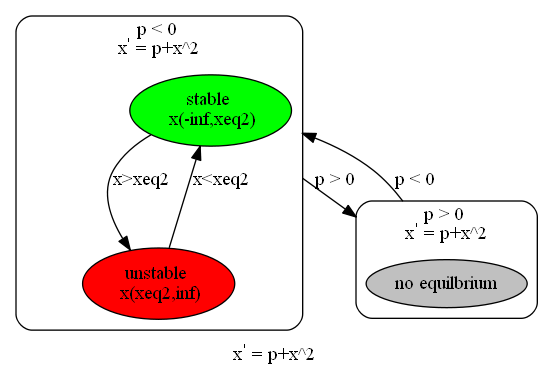
\includegraphics[width=3in]{feb24_graph_sn1.png}
	\caption{Saddle node case}
	\label{feb24_graph_sn1}
\end{subfigure}
\qquad \qquad
\begin{subfigure}[b]{0.4\textwidth}
	\centering
	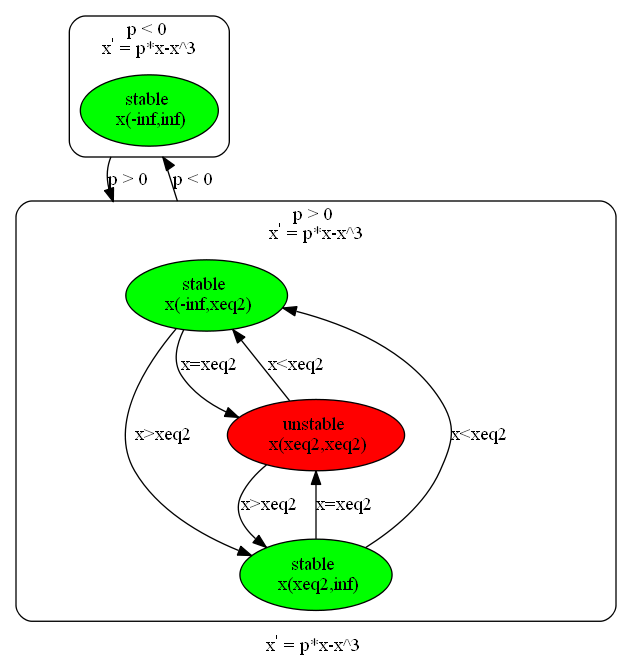
\includegraphics[width=3in]{feb24_graph_pf1.png}
	\caption{Pitchfork case}
	\label{feb24_graph_pf1}
\end{subfigure}
\qquad \qquad
\begin{subfigure}[b]{0.4\textwidth}
	\centering
	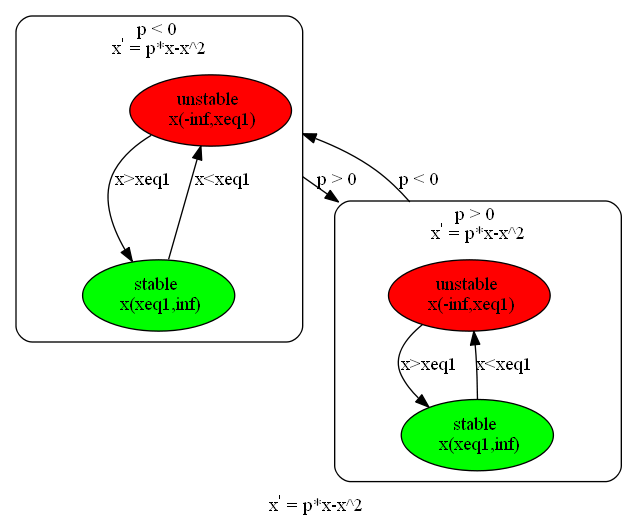
\includegraphics[width=3in]{feb24_graph_tc1.png}
	\caption{Transcritical case}
	\label{feb24_graph_tc1}
\end{subfigure}
\caption{Automated graph representation output for typical bifurcation general cases.}
\label{feb24_graph}
\end{figure}

\subsubsection{Questions/concerns}
\begin{itemize}
\item Some of the modifications required to automate the graph generation of general cases altered the previous structure used for the fixed-$p$ cases. Therefore some simple updates are required to re-enable graph generation for fixed-$p$ cases.
\item As discussed in the previous update, it would be useful to have explicit equations for the solution branches defined by the stable and unstable $x$-nodes. The addition of this feature will be investigated. 
\item With the automated graph generation functional for the 3 prototypical cases, other irreducible systems will be investigated to test the algorithm before proceeding to reducible (i.e. more complex) systems.
\end{itemize}


\subsection{March 3, 2017}
The first version of the automated graph representation algorithm  for irreducible cases has been completed. Since the previous update, issues with the fixed-$p$ cases were addressed. The algorithm was successfully tested on both general and fixed-$p$ cases for the saddle node, pitchfork, and transcritical bifurcations. Figure \ref{mar03_graph_sn} shows the automated outputs for the saddle node case. Note that equilibrium equations have been added to the $x$-nodes. For fixed-$p$ in 1D, this results in a single $x$ value. For example, the stable node in Figure \ref{mar03_graph_sn2} is defined by the equilibrium point $x=-0.7071$ for $p=-0.5$. Therefore, trajectories within the node domain $x\in [-\infty \quad 0.7071]$ will trend towards $x=-0.7071$. This feature is more complicated for general cases since the equilibria are defined by curves instead of points. While COSY produces solution data along these curves, it does not explicitly identify the curve equation. Therefore a symbolic solver was used to determine the equilibrium equations shown in Figure \ref{mar03_graph_sn1}.

\begin{figure}[H]
\centering
\begin{subfigure}[b]{0.4\textwidth}
	\centering
	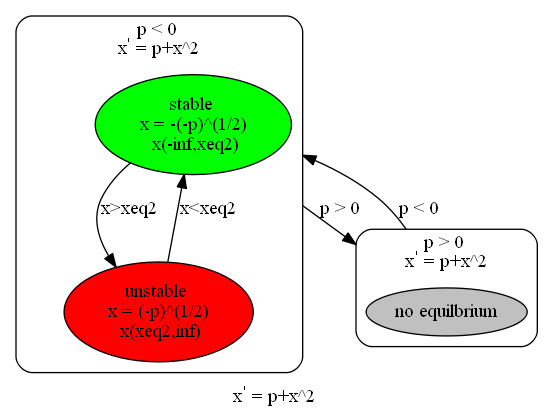
\includegraphics[width=3.75in]{mar03_graph_sn1.png}
	\caption{General $p$}
	\label{mar03_graph_sn1}
\end{subfigure}
\qquad \qquad \qquad
\begin{subfigure}[b]{0.4\textwidth}
	\centering
	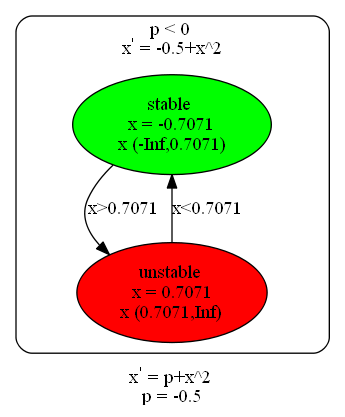
\includegraphics[width=2.25in]{mar03_graph_sn2.png}
	\caption{Fixed $p$}
	\label{mar03_graph_sn2}
\end{subfigure}
\caption{Automated graph representation output for the prototypical saddle node bifurcation general and fixed-$p$ cases.}
\label{mar03_graph_sn}
\end{figure}

\subsubsection{Questions/concerns}
\begin{itemize}
\item While a version of the automated graph process is complete, modifications are expected as this work progresses. This includes needed improvements as more complex systems are investigated and general code cleanup.
\item The symbolic solver method to obtain equilibrium equations for general cases works on the simple systems presented thus far, but identifying these equations will likely become more difficult as more complex systems are investigated.
\end{itemize}


\subsection{March 10, 2017}
An investigation into the graph representation of systems with more complexity than the prototypical bifurcation cases is underway. This has started with multi-parameter systems, where the equation

\begin{equation}
\label{mar10_eq1}
\dot{x}=p_1x+p_2x^2-x^3
\end{equation}
is being used to test the graph representation method. Ideally, the equation \ref{mar10_eq1} system can be represented as subsystem nodes that depend on varying parameter values. While testing the $p_2=1$, varying $p_1$ and $x$ case (i.e. $\dot{x}=p_1x+x^2-x^3$), an issue was encountered in the way that the graph representation algorithm separated the solution branch data. This issue was resolved, and the graph output for this case is shown in Figure \ref{mar10_graph_mp1}, with the COSY bifurcation diagram shown in Figure \ref{mar10_bfd1} for reference.

\begin{figure}[H]
\begin{center}
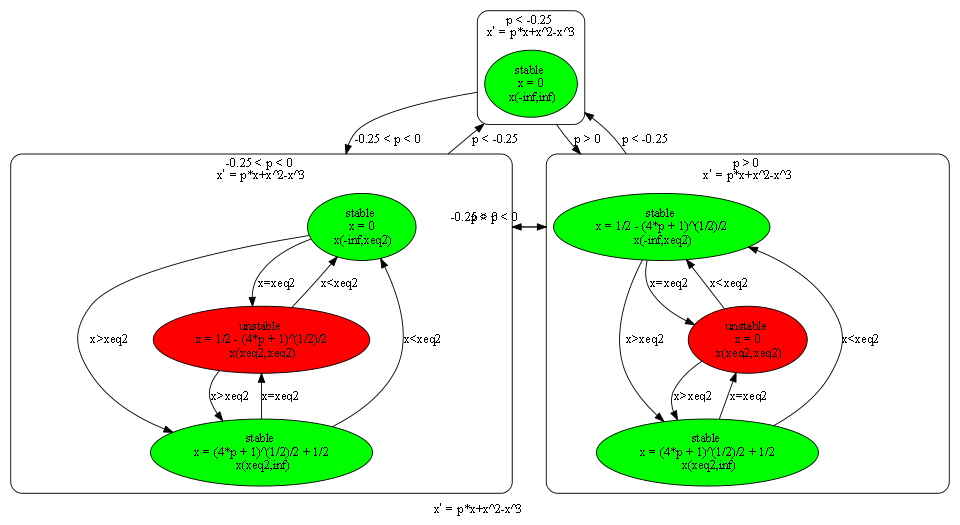
\includegraphics[width=6in]{mar10_graph_mp1.png}
\caption{Graph representation for $\dot{x}=p_1x+x^2-x^3$.}
\label{mar10_graph_mp1}
\end{center}
\end{figure}

\begin{figure}[H]
\begin{center}
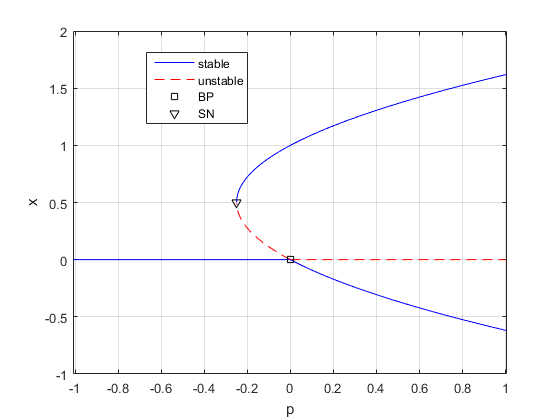
\includegraphics[width=3.5in]{mar10_bfd1.png}
\caption{Bifurcation diagram for $\dot{x}=p_1x+x^2-x^3$.}
\label{mar10_bfd1}
\end{center}
\end{figure}


\subsection{March 24, 2017}
\subsubsection{Transition Scheme}
The automated generation of transition conditions between $x$-nodes has been changed so that only nodes with adjacent domains have transitions between them. Previously, all $x$-nodes had transitions with each other. This change was intended to capture actual behavior. For example, Figure \ref{mar24_graph_pf} shows a fixed-$p$ pitchfork bifrucation case with the old and new transition schemes. The old scheme contained transitions between the two stable nodes, thus neglecting the unstable node at $x=0$ that is crossed when $x$ moves across one stable node to the other. The new scheme instead requires passage through the unstable node to change between the stable nodes. 

\begin{figure}[H]
\centering
\begin{subfigure}[b]{0.4\textwidth}
	\centering
	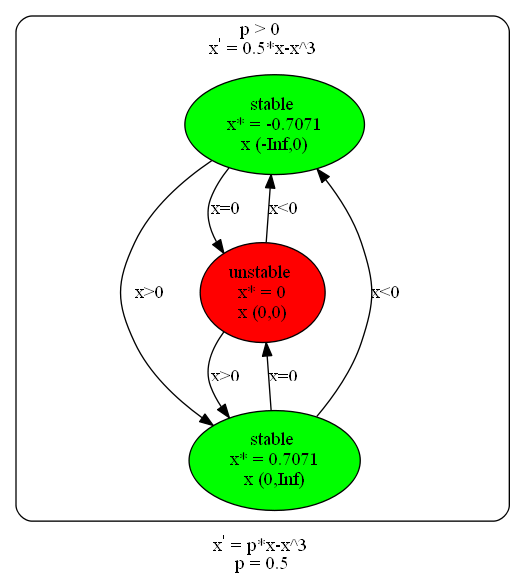
\includegraphics[width=2.5in]{mar24_graph_pf1.png}
\end{subfigure}
\qquad 
\begin{subfigure}[b]{0.4\textwidth}
	\centering
	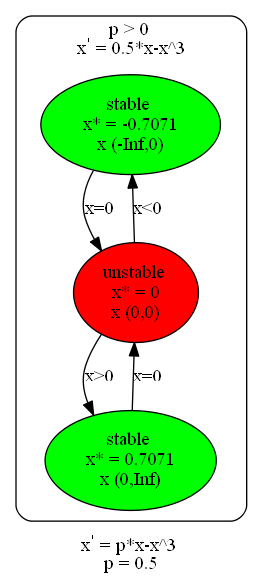
\includegraphics[width=1.25in]{mar24_graph_pf2.png}
\end{subfigure}
\caption{Original (left) and updated (right) transition schemes for a fixed-$p$ pitchfork bifurcation.}
\label{mar24_graph_pf}
\end{figure}

\subsubsection{Executable Function}
The current output of the algorithm is a graph representation PNG image file generated via GraphViz. It is desired to create a function based on the data used to generate the graph representation for system execution. Therefore a preliminary function generator has been created for the irreducible cases using node data. The output function file is organized as a list of if-statements that identifies which $p$ domain the system resides in and applies the relevant dynamics. Currently for the irreducible cases, these dynamics are equivalent since the same dynamics govern the system behavior regardless of $p$ domain. For example, in the saddle-node bifurcation case, $\dot{x}=p+x^2$ defines the governing dynamics regardless of whether $p<0$ or $p>0$. However, this format is expected to capture valuable changes in dynamics as multi-parameter and multi-dimensional systems are explored. Separation of $x$ domains in addition to $p$ domains may also provide useful behavioral distinctions.


\subsubsection{Multi-parameter Systems}
The system

\begin{equation}
\label{mar24_eq1}
\dot{x}=p_1+p_2x+p_3x^2-p_4x^3
\end{equation}
is being used to investigate the graph representation method on multi-parameter, one-dimensional systems. Since numerical continuation requires that the number of unknowns is greater than the number of equations by one, only one parameter (along with the one state, $x$) can be varied at a time for systems such as equation \ref{mar24_eq1}. Therefore to apply the continuation analysis to equation \ref{mar24_eq1}, three of the parameters $p_1,...,p_4$ must be set as constants for a single continuation process. This process can then be repeated with different designations of interest for $p_1,...,p_4$. 

To capture continuation processes with varying parameter designations, a ``top'' layer of nodes was added to the graph representation scheme. Each of these nodes are defined by different sets of parameter designations that form subsets of the top level dynamics describe by equation \ref{mar24_eq1}. For reference, the ordering of nodes starting from the top is now: top-node, $p$-node, and $x$-node. The current coloring scheme displays top-nodes as tan, $p$-nodes as white, and $x$-nodes as green/red/grey, depending on stability. As an example, the three parameter designations for equation \ref{mar24_eq1},

\begin{equation}
\begin{split}
1: \quad p_1=p, \quad p_2=0, \quad p_3=0, \quad p_4=1 \\ 2: \quad p_1=0, \quad p_2=p, \quad p_3=0, \quad p_4=1 \\ 3: \quad p_1=p, \quad p_2=0, \quad p_3=1, \quad p_4=0
\end{split}
\end{equation}
where $p$ without a subscript denotes the active continuation parameter, define three separate top-nodes. The resulting dynamic subsets are

\begin{equation}
\begin{split}
1: \quad \dot{x}=p-x^3 \\ 2: \quad \dot{x}=px-x^3 \\ 3: \quad \dot{x}=p+x^2.
\end{split}
\end{equation}
The output for general and example fixed-$p$ cases are shown in Figure \ref{mar24_graph_mp}. 

\begin{figure}[H]
\centering
\begin{subfigure}[b]{0.4\textwidth}
	\centering
	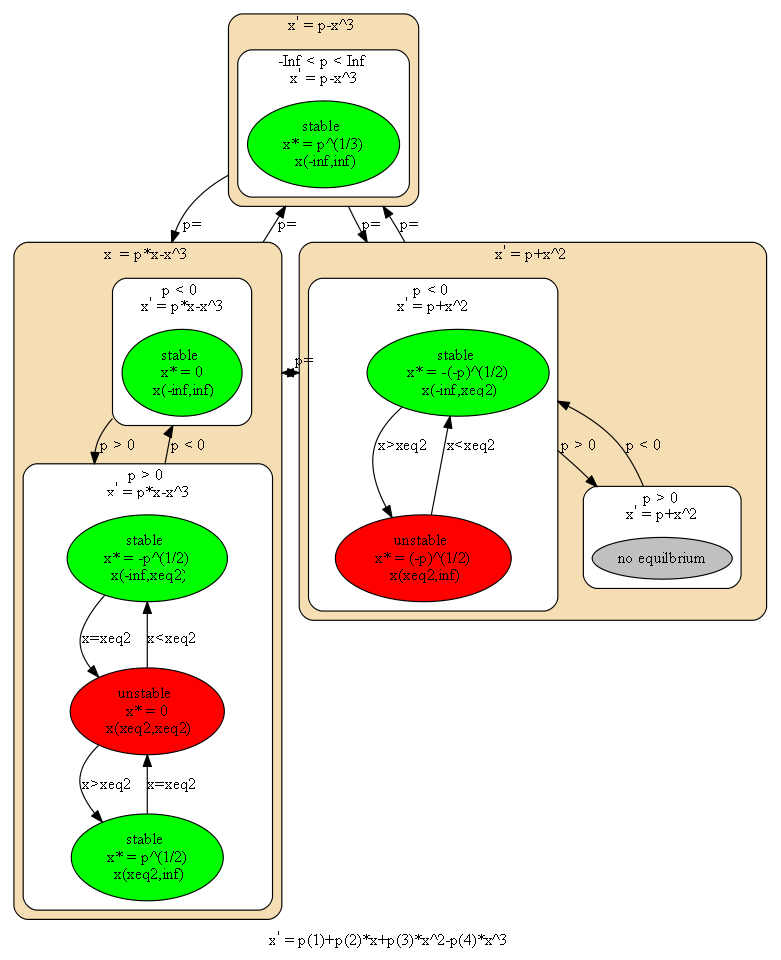
\includegraphics[width=3.5in]{mar24_graph_mpgen.png}
	\caption{General $p$}
\end{subfigure}
\qquad \qquad \qquad
\begin{subfigure}[b]{0.4\textwidth}
	\centering
	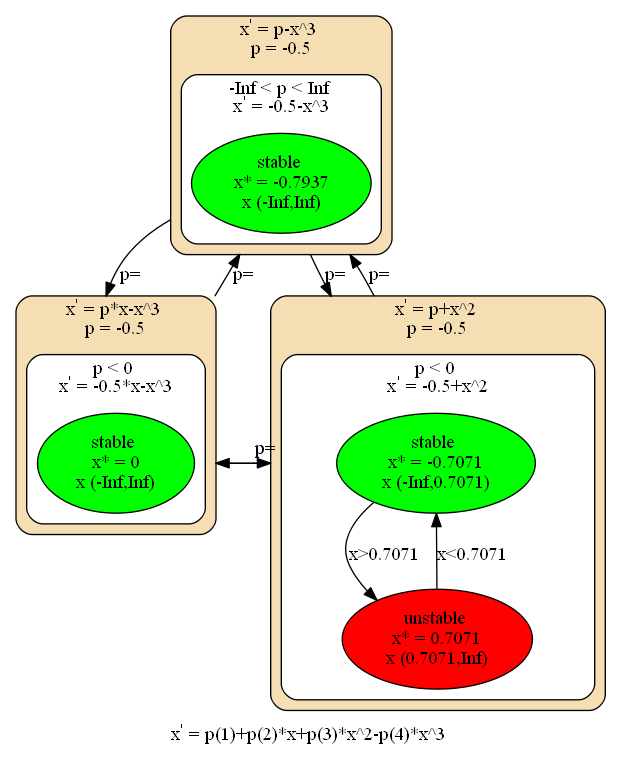
\includegraphics[width=3in]{mar24_graph_mpfp.png}
	\caption{Fixed $p$}
\end{subfigure}
\caption{Graph representation of $\dot{x}=p_1+p_2x+p_3x^2-p_4x^3$ with three different parameter designations.}
\label{mar24_graph_mp}
\end{figure}

Figure \ref{mar24_graph_mp} was generated automatically by modifying the graph representation algorithm so that it can process multiple sets of COSY output data. However, the three sets of data used were created by manually running three COSY processes. A separate process is proposed where the user identifies the top level dynamics and a parameter designation matrix, with each row defining a subset and each column a parameter. Then, an automated process would generate the subset dynamics, run COSY on each subset, and send the resulting data to the automated graph representation algorithm.


\subsubsection{GitHub Repository}
A GitHub repository (\texttt{https://github.com/pcouth/continuation-VV}) has been created for this work. It currently contains:

\begin{itemize}
\item Documentation folder with this report and archived reports
\item Tools folder with GraphViz
\item Examples folder with the 1-parameter, 1-dimensional graph representation code, COSY data output files for three prototypical bifurcation cases, and a script that runs the graph representation for the prototypical examples
\end{itemize}


\subsubsection{Questions/concerns}
\begin{itemize}
\item The multi-parameter graph representation is incomplete. Top-node transition conditions need to be added. Top-nodes should also contain parameter conditions (e.g. $p_2=p_3=0, p_4=1$). Currently, the varied parameter within each top-node is labeled $p$. It would be useful to label these as $p_1,p_2,...$ in order to track which parameter from the original dynamics is being varied.
\item The proposed algorithm for generating multiple COSY data sets of multi-parameter systems needs to be created.
\item Modifications are required to produce executable functions for multi-parameter systems.
\end{itemize}


\begin{thebibliography}{9}

\bibitem{allgower}
Allgower, E. L. and Georg, K., {\it Introduction to Numerical Continuation Methods}, Society for Industrial and Applied Mathematics, Philadelphia, PA, 1990.

\bibitem{Strogatz}
S. Strogatz, Nonlinear Dynamics and Chaos with Applications to Physics, Biology, Chemistry, and Engineering, Westview Press, 2nd edition, 2015.

\bibitem{spetzler}
Spetzler, M. G., and Narang-Siddarth, A., "Continuation Analysis of Nonlinear Systems with Equality Constraints on States, Parameters, and Eigenvalues," {\it AIAA Guidance, Navigation and Control Conference}, AIAA Paper 2015-1320, 2015, doi: 10.2514/1.C031247

\bibitem{Clarke1}
E. M. Clarke, E. A. Emerson and A. P. Sistla. Automatic verification of finite-state concurrent systems using temporal logic specifications. In ACM Transactions on Programming Languages and Systems, 8(2):244--263, 1986.

\bibitem{Clarke2}
E.M. Clarke and Q. Wang. 25 Year of Model Checking: History, Achievement, Perspectives. Springer-Verlag Berlin, Heidelberg, 2008.

\bibitem{Clarke3}
E. M. Clarke, O. Grumberg, and D. E. Long. Model checking and abstraction. In Proceedings of the Nineteenth Annual ACM Symposium on Principles of Programming Languages, January 1992.

\bibitem{Merz}
S. Merz, Model Checking: A Tutorial Overview, Modeling and Verification of Parallel Processes of the series Lecture Notes in Computer Science Volume 2067, pp.3-38, 2001.

\bibitem{Hasan}
O. Hasan and S. Tahar. Formalized Probability Theory and Applications Using Theorem Proving. IGI Global, 2015.

\bibitem{Harrison}
J. Harrison. Handbook of practical logic and automated reasoning. Cambridge University Press, 2009.

\bibitem{Koutsofios}
E. Koutsofios and S. North, \textit{Drawing Graphs with DOT}, Murray Hill, NJ: AT\&T Bell Laboratories, 1996. 

\bibitem{Ellson}
J. Ellson, E. Gansner, E. Koutsofios, S. North and G. Woodhull, ``Graphviz and Dynagraph - Static and Dynamic Graph Drawing Tools,'' AT\&T Lab - Research, Florham Park, NJ, 2003.

\end{thebibliography}


\end{document}
